\paragraph{Thực nghiệm với Flowers-102} \hfill \\
Bộ dữ liệu chứa hình ảnh của các loài hoa phổ biến. Thách thức của bài toán này nằm ở sự tương đồng về màu sắc và cấu trúc giữa các loài hoa khác nhau.

\paragraph{Phân tích Dữ liệu và Tiền xử lý} \hfill \\
Việc quan sát sự phân bổ dữ liệu cho thấy một số loài hoa có số lượng ảnh áp đảo, điều này đòi hỏi mô hình phải có khả năng học đặc trưng tốt để không bị overfit vào các lớp phổ biến.

\begin{figure}[H]
    \centering
    \begin{minipage}{0.48\textwidth}
        \centering
        
\includegraphics[width=\linewidth]{Chương_2/results/flowers/01_class_distribution.png}
        \caption{Phân bổ dữ liệu các loài hoa}
        \label{fig:flowers_dist}
    \end{minipage}
    \hfill
    \begin{minipage}{0.48\textwidth}
        \centering
        
\includegraphics[width=\linewidth]{Chương_2/results/flowers/02_sample_images.png}
        \caption{Hình ảnh mẫu từ Flowers-102}
        \label{fig:flowers_samples}
    \end{minipage}
\end{figure}

\paragraph{MobileNetV2 và Transfer Learning} \hfill \\
Chúng ta sử dụng MobileNetV2 - một kiến trúc sử dụng tích chập tách biệt theo chiều sâu (Depthwise Separable Convolutions). Mô hình chỉ có \textbf{2,592,325} tham số, cực kỳ nhẹ nhưng vẫn mang lại hiệu suất mạnh mẽ. Bằng cách sử dụng Transfer Learning từ ImageNet, mô hình đã thừa hưởng khả năng nhận diện các hình khối và màu sắc cơ bản.

\paragraph{Kết quả thực nghiệm} \hfill \\
Mô hình đạt độ chính xác ấn tượng là \textbf{86.51\%} trên tập kiểm tra.

\begin{figure}[H]
    \centering
    \begin{minipage}{0.48\textwidth}
        \centering
        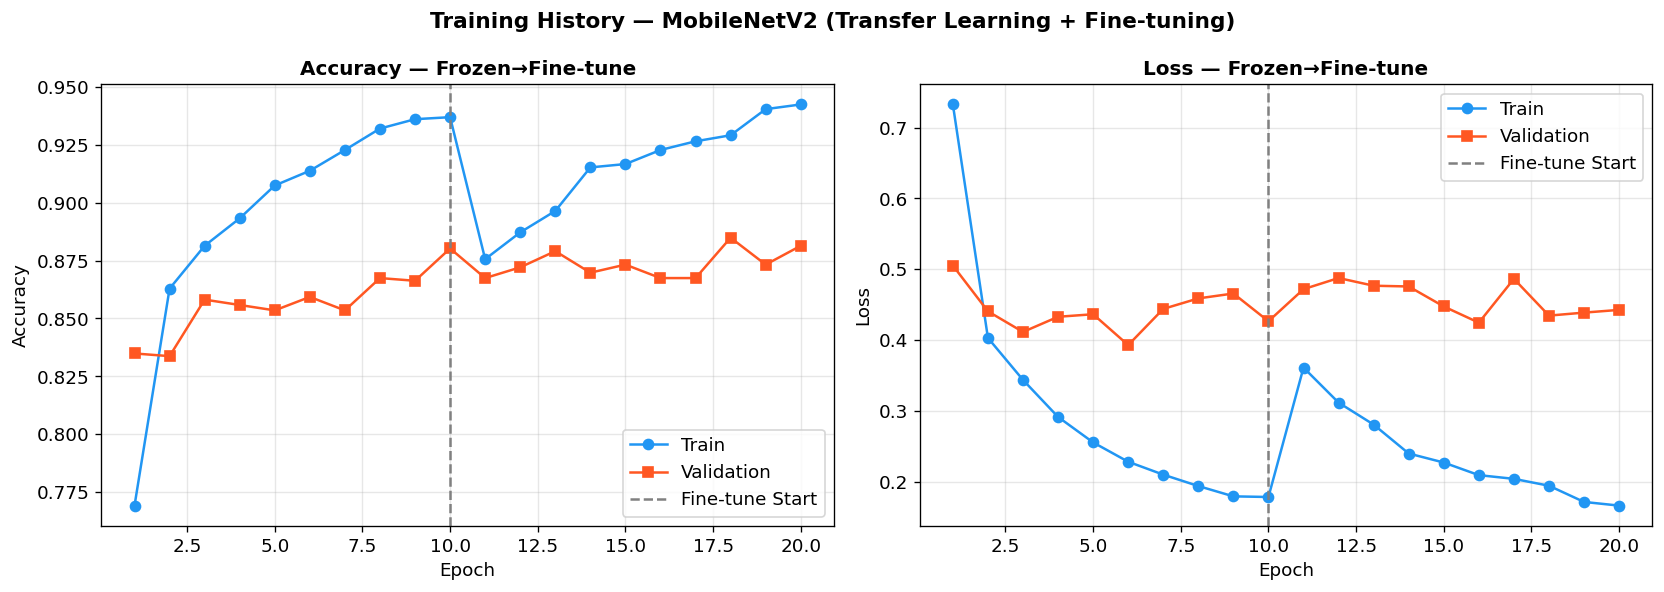
\includegraphics[width=\linewidth]{Chương_2/results/flowers/03_training_history.png}
        \caption{Lịch sử huấn luyện MobileNetV2}
        \label{fig:flowers_history}
    \end{minipage}
    \hfill
    \begin{minipage}{0.48\textwidth}
        \centering
        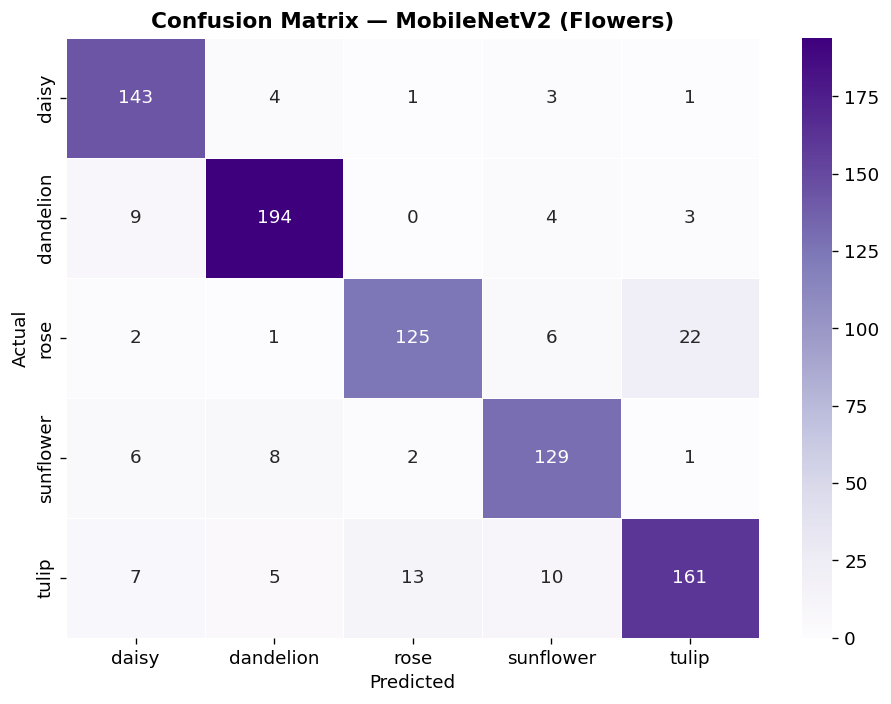
\includegraphics[width=\linewidth]{Chương_2/results/flowers/04_confusion_matrix.png}
        \caption{Ma trận nhầm lẫn phân loại hoa}
        \label{fig:flowers_cm}
    \end{minipage}
\end{figure}

Sử dụng Transfer Learning giúp mô hình không chỉ đạt độ chính xác cao mà còn hội tụ rất nhanh (chỉ sau khoảng 10-15 epoch), tiết kiệm đáng kể tài nguyên tính toán.
